% Created 2020-06-01 Mon 09:49
% Intended LaTeX compiler: pdflatex
\documentclass[presentation]{beamer}
\usepackage[utf8]{inputenc}
\usepackage[T1]{fontenc}
\usepackage{graphicx}
\usepackage{grffile}
\usepackage{longtable}
\usepackage{wrapfig}
\usepackage{rotating}
\usepackage[normalem]{ulem}
\usepackage{amsmath}
\usepackage{textcomp}
\usepackage{amssymb}
\usepackage{capt-of}
\usepackage{hyperref}
\usetheme{UoB}
\author{Mark Blyth}
\date{\textit{[2020-05-25 Mon]}}
\title{Spring project summary}
\hypersetup{
 pdfauthor={Mark Blyth},
 pdftitle={Spring project summary},
 pdfkeywords={},
 pdfsubject={},
 pdfcreator={Emacs 26.3 (Org mode 9.1.9)}, 
 pdflang={English}}
\begin{document}

\maketitle

\section{Previous}
\label{sec:org2c57db8}
\begin{frame}[label={sec:org195a749}]{Last meeting}
Discussion about single-cell and multi-cell approaches
\vfill
Single-cell: 
\begin{itemize}[<+->]
\item Strong literature precedent for what to expect
\item Lots of accepted models to test \emph{in-silico}
\item Easy-to-spot bifurcations
\begin{itemize}
\item Hopf, fold both easily detectable with CBC
\end{itemize}
\item Reuse Bath single-cell microfluidics device
\end{itemize}
\end{frame}


\begin{frame}[label={sec:orgd2e8c53}]{Last meeting}
Discussion about single-cell and multi-cell approaches
\vfill
Multi-cell: 
\begin{itemize}[<+->]
\item Assume there's an arbitrarily large number of cells
\begin{itemize}
\item Neural continuum fields (limited descriptive ability)
\item Spatially extended cubic Lienard system
\end{itemize}
\item Search experimentally and numerically for PDE bifurcations
\begin{itemize}
\item Not an area I know much about (yet\ldots{})
\end{itemize}
\item Can build on work by Krasi's Munich collaborators
\item Or could reuse Bath microfluidic device
\begin{itemize}
\item Would require minor alterations to increase spatial resolution
\end{itemize}
\end{itemize}
\end{frame}


\begin{frame}[label={sec:orgf004362}]{Single- vs multi-cell}
Deciding factors:

\vfill

\begin{itemize}
\item No lab access for the forseeable future
\begin{itemize}
\item Work can be guided less by experiments
\end{itemize}
\item Single-cell easier than multi-cell
\begin{itemize}
\item I know enough about single-cell CBC to start working on it
\end{itemize}
\end{itemize}

\vfill

Conclusion: work on single-cell case
\end{frame}


\section{Current}
\label{sec:org97e4509}
\begin{frame}[label={sec:orgcf579b1}]{Current goals}
\begin{itemize}
\item Single-cell \emph{in-silico} CBC
\item Tutorial-review paper for numerical continuation
\end{itemize}
\end{frame}

\begin{frame}[label={sec:orga80a685}]{Challenges of \emph{in-silico} CBC}
Data aren't ideal to work with:
\vfill
\begin{itemize}
\item Real signals are noise-corrupted
\begin{itemize}
\item Difficult to filter off, since spikes contain lots of high-frequency components
\item Hard to run continuation on stochastic and noisy signals
\end{itemize}
\end{itemize}
\vfill
\begin{itemize}
\item Neurons are fast-spiking
\begin{itemize}
\item Fourier discretisation won't work
\item Discretisations need to be very high-dimensional, making Jacobian very slow to find
\end{itemize}
\end{itemize}

\vfill
\end{frame}

\begin{frame}[label={sec:org2e93256}]{Issue 1: noise corruption}
Instead of running continuation on noisy signal measurements, let's run it on a surrogate data source
\begin{itemize}[<+->]
\item Assume no knowledge of the system
\begin{itemize}
\item CBC is a model-free method
\end{itemize}
\item Come up with some surrogate model to replace the observed data
\begin{itemize}
\item Must filter out the noise
\item Must handle experimental issues (missing measurements, uneven spacing, small amounts of data)
\end{itemize}
\item Surrogate model can then be analysed as desired
\begin{itemize}
\item Smooth, clean datasource (no noise, no missing points, full interpolation)
\item Accurate derivatives, of arbitrary order
\item Allows for accurate delay embeddings, collocation discretisation -- conventional continuation can be used on it
\end{itemize}
\end{itemize}

\vfill
\end{frame}

\begin{frame}[label={sec:orgee407e3}]{Candidate surrogate models}
\begin{itemize}[<+->]
\item Truncated Fourier series
\begin{itemize}
\item Currently used in CBC
\item Bad for noisy or spiking data
\end{itemize}
\item Wavelet decomposition
\begin{itemize}
\item `Enveloped' oscillations
\end{itemize}
\item Splines
\begin{itemize}
\item Piecewise-polynomial model
\end{itemize}
\item Gaussian process regression
\begin{itemize}
\item Statistically optimal, when noise is Gaussian
\end{itemize}
\end{itemize}

These require no preexisting knowledge \emph{[loosely speaking]}, and work well with sparse data
\end{frame}

\begin{frame}[label={sec:org745afa2}]{Gaussian process regression}
\begin{center}
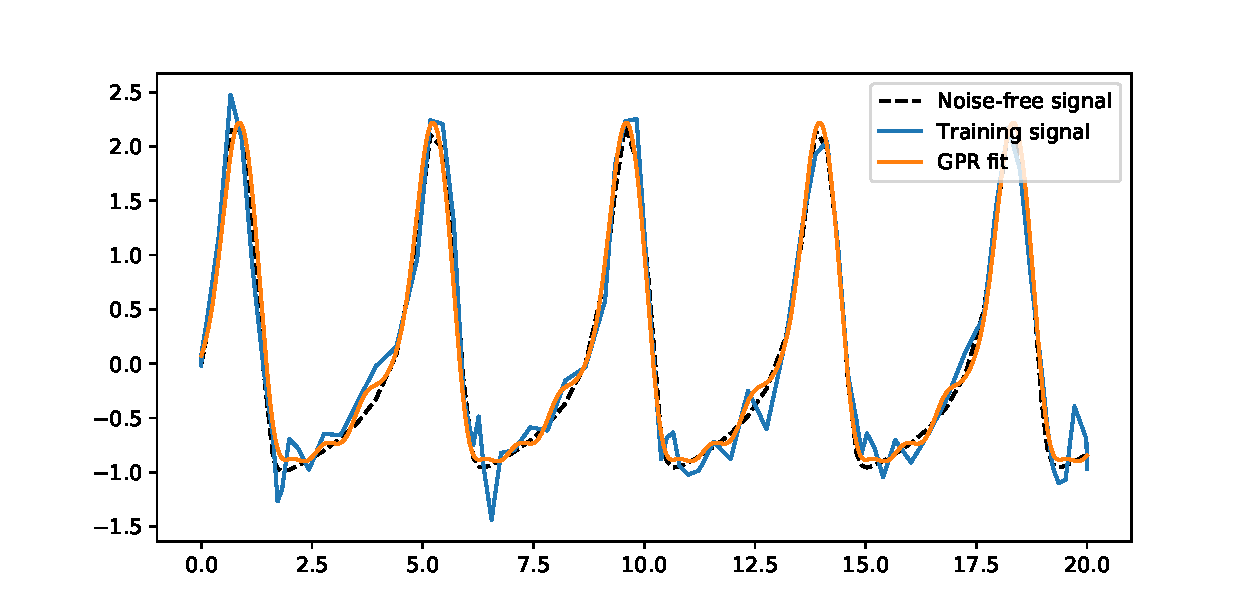
\includegraphics[width=.9\textwidth]{./GPR_demo.pdf}
\end{center}

GPR can recover the underlying signal from noise-corrupted observations
\end{frame}

\begin{frame}[label={sec:orgedf2408}]{Surrogate models}
\begin{center}
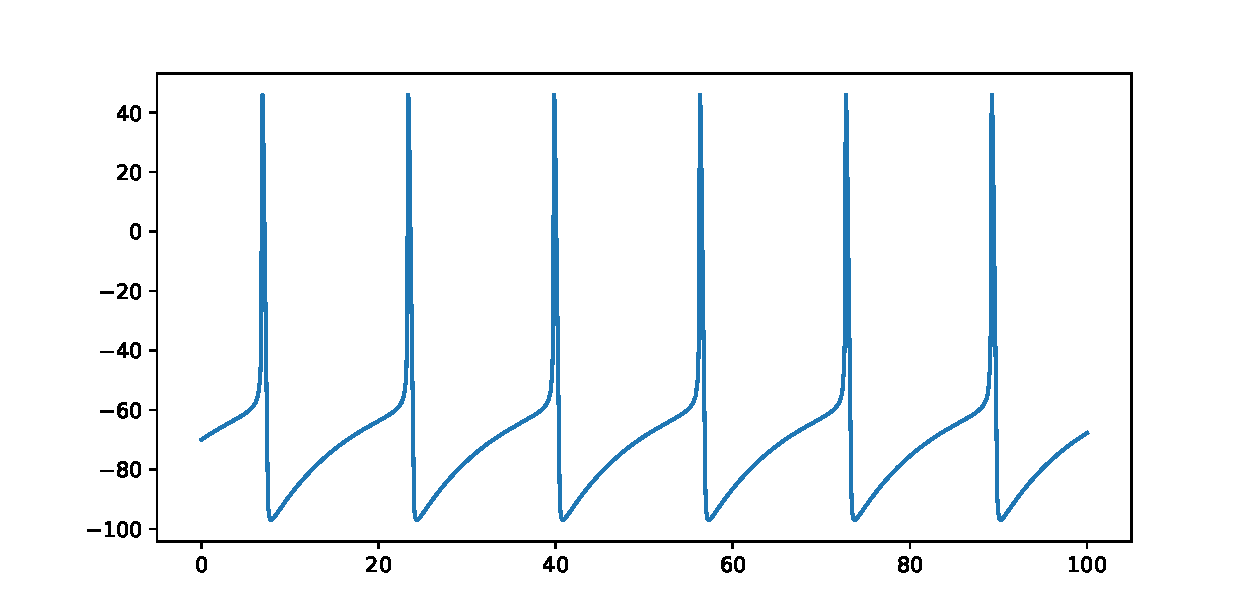
\includegraphics[width=.9\textwidth]{./HHraw.pdf}
\end{center}

GP surrogate models don't always work well!
\end{frame}

\begin{frame}[label={sec:orgd9932a3}]{Surrogate models}
\begin{center}
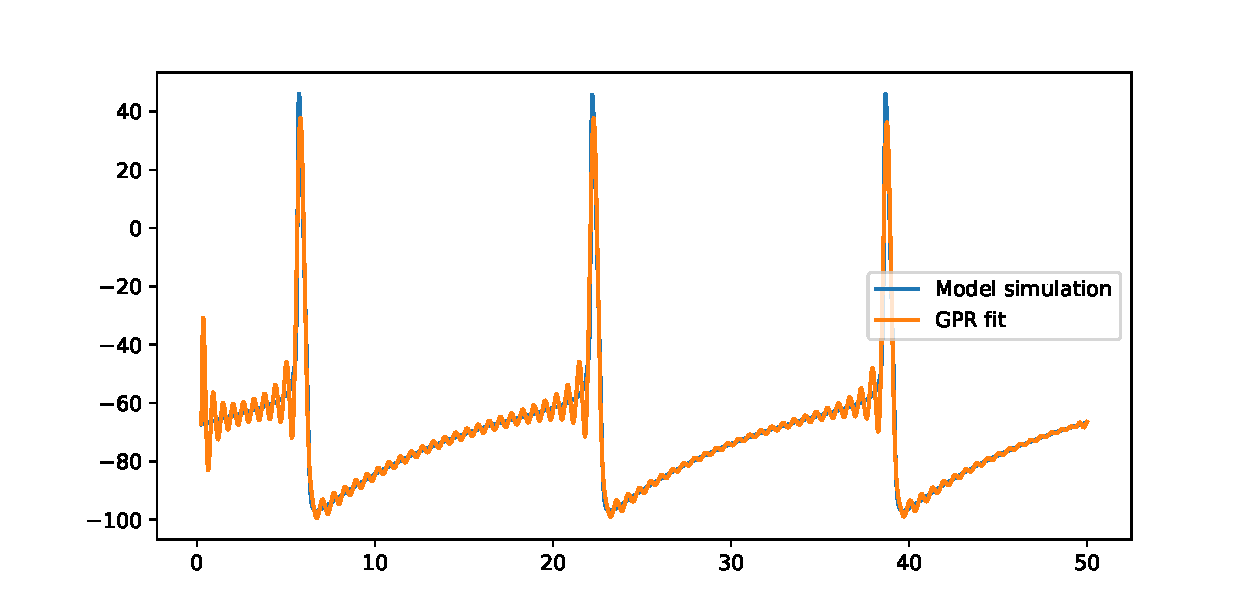
\includegraphics[width=.9\textwidth]{./HH_FKL_test.pdf}
\end{center}
GP surrogate models don't always work well!
\end{frame}

\begin{frame}[label={sec:org35be246}]{Machine learning for dynamical systems}
\begin{itemize}[<+->]
\item Current approach: Gaussian process regression; predict new points as an intelligently weighted sum of example points
\item Bayesian kernel method
\begin{itemize}
\item Kernel specifies a distribution over basis functions
\item Good kernel choice = good data fit
\end{itemize}
\item Most kernels are stationary
\begin{itemize}
\item Assumes statistical properties are time-invariant \emph{[they're not]}
\item Can't handle the spiking behaviours of neurons
\end{itemize}
\end{itemize}

\vfill

Current goal: find a good approach to fitting a surrogate model
\end{frame}


\section{Next}
\label{sec:orgf548bb9}

\begin{frame}[label={sec:org2157b55}]{Next questions}
\begin{itemize}
\item Surrogate models on real data
\item Predictor-corrector design
\item Stochastic models
\end{itemize}
\end{frame}

\begin{frame}[label={sec:org621bd50}]{Continuation issues}
\begin{itemize}
\item Discretisation is required to make predictor-corrector methods work
\begin{itemize}
\item Can't run continuation on a function; must discretise it into a vector
\end{itemize}
\item Discretisation has issues when used on fast-spiking data
\begin{itemize}
\item Requires lots of datapoints
\item Slow to find a Jacobian for Newton-iterations
\item High noise-sensitivity
\end{itemize}
\item Surrogate models and discretisation-free predictor-correctors might help overcome these
\end{itemize}
\end{frame}

\begin{frame}[label={sec:orge747583}]{Alternative continuation approach}
Predictor-corrector design:
\vfill
\begin{itemize}
\item We could try discretisation-free predictor steps, using a surrogate model
\begin{itemize}
\item Let \(f_i(t)\) be the surrogate model for system behaviours at parameter \(\lambda_i\)
\item Given periodic orbits \(f_{i-1},~f_i\), predict \(f_{i+1} = f_i + h \big[f_i - f_{i-1}\big]\)
\end{itemize}
\end{itemize}
\vfill
\begin{itemize}
\item Corrector step would be harder
\end{itemize}
\end{frame}

\begin{frame}[label={sec:org764dcc9}]{Stochastic models}
Another challenge: real neurons are stochastic
\vfill
\begin{itemize}
\item Stochasticity introduces new challenges
\begin{itemize}
\item Coherence and stochastic resonance
\item Random attractors
\item Stochastic calculus
\item Not an area I know much about \emph{[yet\ldots{}]}
\end{itemize}
\item Current work: CBC on noise-corrupted simulations
\item Next work: CBC on truly stochastic models
\end{itemize}

\vfill

Big question: how different would truly stochastic models be?
\end{frame}


\begin{frame}[label={sec:org37f5b1e}]{Goals}
Actions:
\begin{itemize}
\item Find a surrogate modelling method for neural data
\item Attempt a discretisation-free corrector?
\item Run CBC on deterministic models, then stochastic
\end{itemize}

\vfill

Results:
\begin{itemize}
\item Write up surrogate modelling into a conference abstract \emph{[July]}
\begin{itemize}
\item Maybe a conference paper \emph{[September]}
\end{itemize}
\item Use surrogate modelling for an \emph{in-silico} CBC paper \emph{[next year?]}
\end{itemize}
\end{frame}


\section{Normal supervision slides}
\label{sec:orgf75e015}
\begin{frame}[label={sec:org57a9471}]{BONUS: Week's work}
\begin{itemize}[<+->]
\item Functional kernel learning now works
\begin{itemize}
\item Stationary kernel method
\item Performs well on Fitzhugh-Nagumo
\item Performs badly on Hodgkin-Huxley
\end{itemize}
\item New model validation method
\begin{itemize}
\item Run a high-accuracy solver, for lots of datapoints
\item Downsample
\item Train models on half the datapoints, test them on the other half
\item Could optionally do an error integral, since we have a continuous model
\end{itemize}
\item Looked into noise-training
\begin{itemize}
\item Couldn't find anything
\end{itemize}
\item Non-stationary kernel is not working
\item Support vector regression
\end{itemize}
\end{frame}

\begin{frame}[label={sec:org03b9887}]{BONUS: SVR}
\begin{itemize}[<+->]
\item SVR is the regression-equivalent of a support vector machine
\begin{itemize}
\item Another popular kernel method
\end{itemize}
\item It works moderately well on neuron data
\begin{itemize}
\item Fast!
\item Fair performance on non-stationary data
\item Doesn't always average out noise well
\end{itemize}
\item Another idea: ensemble models
\begin{itemize}
\item Fit a few different models (GPR, splines, SVR, etc)
\item Use something analogous to sensory fusion, to combine model predictions
\item Gradient boosting: combine several weak learners to make a single strong learner
\end{itemize}
\end{itemize}

Only worth trying after I've tested all the other regression methods
\end{frame}

\begin{frame}[label={sec:org779d04b}]{BONUS: SVR}
\begin{center}
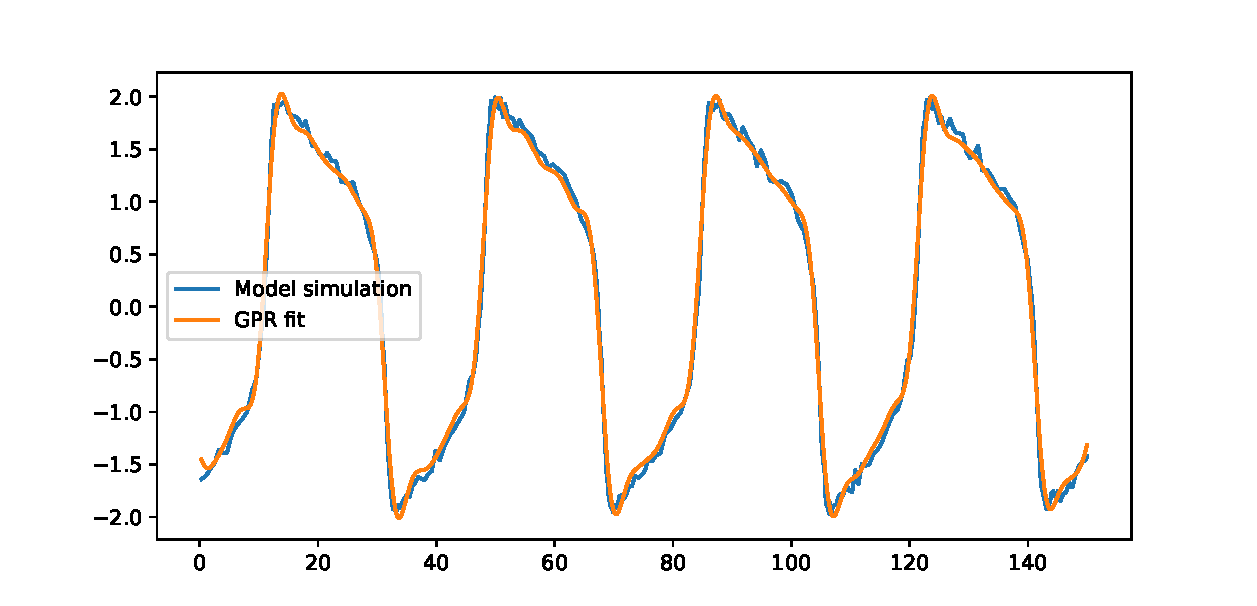
\includegraphics[width=\textwidth]{./SVR.pdf}
\end{center}
\end{frame}
\end{document}
